\documentclass{homework}
\author{Witninger, Caleb}
\class{CSCI 2114: Tashfeen's Data Structures}
\date{\today}
\title{Homework 1}
\address{%
  Oklahoma City University, %
  Petree College of Arts \& Sciences, %
  Computer Science%
}

\acmfonts
\newcommand\callit[1]{Store the code in a file called \texttt{#1}.}
\newcommand\docs{\href{%
    https://tinyurl.com/25w2e4wy%
  }{%
    \texttt{Byte.toUnsignedInt(byte x)}%
  }%
}

\begin{document} \maketitle

\question Briefly define the following terms in context of computer
hardware.

\begin{enumerate}
  \item Register
  \item Memory
  \item Disk
\end{enumerate}

\begin{sol}
 1 - A register is an area where data being processing is stored that on a CPU. They are most commonly found in 32 or 64 bit sizes \smallbreak
 2 - Typically refers to RAM storage on a computer where temporary data is stored while in use. Short term memory.\smallbreak
 3 - Disk -  
   Refers to the hardrive of the computer where data is stored or long term use. Long term memory\smallbreak
\end{sol}

\question What is the smallest addressable unit of memory in most modern
computers?

\begin{sol}
Bytes are typically the smallest addressable units of memory because computers group data into that size
\end{sol}

\question Give the number of bytes in the following memory units as either 2
or 10 raised to an appropriate power. For example, a Kibibyte
(KiB) is $2^{10}$ bytes while a Kilobyte (KB) is $10^3$ bytes.

\begin{enumerate}
  \item Mebibyte (MiB)
  \item Megabyte (MB)
  \item Gibibyte (GiB)
  \item Gigabyte (GB)
  \item Tebibyte (TiB)
  \item Terabyte (TB)
  \item Pebibyte (TiB)
  \item Petabyte (TB)
\end{enumerate}

\begin{sol}
1. MiB - $2^{20}$ \smallbreak
2. MB - $10^{6}$ \smallbreak
3. GiB - $2^{30}$ \smallbreak
4. GB - $10^{9}$ \smallbreak
5. TiB - $2^{40}$ \smallbreak
6. TB - $10^{12}$ \smallbreak
7. PiB - $2^{50}$ \smallbreak
8. PB - $10^{15}$ \smallbreak
\end{sol}

Why is there a need for two byte-prefixed unit systems?\smallbreak
\begin{sol}
The binary base 2 measurements are based on the actual amount of bytes in a medium, while the decimal base 10 measurements are easier for humans to read and understand
\end{sol}

\question Java class in listing \ref{types} prints the maximum numerical
value each Java primitive type can store. Explain how these are
calculated \ie their connection to register size and numerical
sign. \bigbreak

\begin{sol}
Byte's max decimal is equal to $(2^{8-1})-1$. This is because there are 8 bits in a byte and one is used for
negativity $(8-1)$. The number could be 0 so we include the -1 to account for that. \bigbreak

A short is equal to $(2^{16-1})-1$, two bytes of data / 16 bit signed \bigbreak

A char is $(2^{16})-1$ since its unsigned/always positive. 16 bit unsigned \bigbreak

Int is $(2^{31})-1$. 32 bit signed \bigbreak

Long is 64 bit signed \bigbreak

A float is a 32 bit data type where there is 1 sign bit, 8 control the scale of the number as an exponent, 
and 23 are the actual number although decimals 0 and 255 are reserved.The formula comes out to 
$(2-2^{-23})*2^{127}$. \bigbreak

Double has 1 sign bit, 11 scale bits, and 52 number bits and equals $(2-2^{-52})*2^{1023}$ \bigbreak

32 bit cpus can still run operations on 64 bit data types but are less efficient
\end{sol}

% \lstinputlisting[
%   language={java},
%   caption={Java class to print maximum values of primitive types.},
%   label=types]
% {code/Constants.java}

\question Write a Java program that prints out one line of text to the
console. It can be anything but ``Hello World!'' What did you
print? \callit{Anything.java}

\begin{sol}
  "Goodbye Space!"
\end{sol}

\question Write a Java program that populates an array of size $n$ with the
first $n$ Fibonacci numbers. The program should print out the
array as shown in figure \ref{exmp}. Here $n$ should be the first
command line argument. You may do it anyway you like but one and
arguably the most elegant way to do it is recursively as shown in
the listing \ref{fib}. What is the name of the implicit call
structure that is used in listing \ref{fib}? Hint: Stack Overflow.
\callit{Fibonacci.java}

\begin{sol}
Call Stack
\end{sol}

% \lstinputlisting[
%   linerange={22-26},
%   language={java},
%   caption={Java function to generate the Fibonacci sequence.},
%   label=fib]
% {code/Fibonacci.java}

\question Using the
\href{https://en.wikipedia.org/wiki/Sieve_of_Eratosthenes}{Sieve
  of Eratosthenes}, populate a boolean array of size $n$ (Java
booleans initialise to false) marking all the indices that are
Composite numbers to true. Here $n$ should be the first command
line argument. The indices remaining false at the end should be
Prime numbers. \callit{Eratosthenes.java}

\begin{enumerate}
  \item For debugging, have your program print all the prime numbers less
        than a 100. You should get the following: $ 2, 3, 5, 7, 11, 13,
          17, 19, 23, 29, 31, 37, 41, 43, 47, 53, 59, 61, 67, 71, 73, 79,
          83, 89, 97. $

          \begin{sol}
            97 89 83 79 73 in 1.0965E-5 seconds
          \end{sol}
  \item The program should print out at most the five largest prime
        numbers it computed and the time (seconds) it took to compute all
        the primes less than $n$. Here is a way to compute seconds taken
        by a function call \texttt{eratosthenes(toSieve)}.

        \begin{lstlisting}[language=java]
double startTime = System.nanoTime();
eratosthenes(toSieve);
double duration = System.nanoTime() - startTime;
duration = duration / Math.pow(10, 9);
\end{lstlisting}

  \item With your program, calculate how long does it take (in seconds) to
        compute all the 30 bit prime numbers. These are all primes less
        than $n = 2^{30} = 1073741824$.

        \begin{sol}
          1073741789 1073741783 1073741741 1073741723 1073741719 in 18.236022787 seconds
        \end{sol}

  \item Can your implementation of the Sieve of Eratosthenes compute all
        the 32 bit prime numbers? If yes, give the time it takes or if it
        can not, then why not?

        \begin{sol}
          No, i used an int for n and int is a 32 bit signed data type so it cannot store the decimal $2^{32}$. Also, arrays use int for the index and has the same limit on length.
        \end{sol}
\end{enumerate}

\question\label{32bitprimes} Read all bytes in the file
\href{https://tinyurl.com/24bvsnaf}{\texttt{half\_gaps.bin}}. You may
use the function in code listing \ref{byte}.

% \lstinputlisting[
%   linerange={36-44},
%   language={java},
%   caption={Java function to read in a file's (signed) bytes.},
%   label=byte]
% {code/Primes.java}

The function in code listing \ref{byte} reads in signed bytes.
While this maybe suitable for some binary arrangements, we want
the bytes to be unsigned. One way to achieve this is to just loop
and use \docs{} as seen in listing \ref{long}.

% \lstinputlisting[
%   linerange={9-13},
%   language={java},
%   caption={Converting Java signed bytes to unsigned longs.},
%   label=long]
% {code/Primes.java}

Compute the array of integers' cumulative sum \ie
\[
  \curl{x_i \in \mathtt{cumsum}(x) : x_i = \sum_{k=1}^{i} x_k}
\]
Now multiply each of the sums with 2 and then add a 3.
\[
  \curl{x_i \in \mathtt{cumsum}(x) :
    y_i = 2x_i+3 = 2\paren{\sum_{k=1}^{i} x_k}+3}
\]
\begin{enumerate}
  \item Print out the first fifteen and the last five elements of this
        final array.
  \item Time this program (the reading of bytes, the cumulative sum
        computation and the doubling with adding a three) and print the
        result in seconds.
  \item Do you recognise the printed numbers? What will these be if we
        further prepended a 2 and a 3 to them?
\end{enumerate}

\begin{sol} \smallbreak
2 \smallbreak
3 \smallbreak
5 \smallbreak
7 \smallbreak
11 \smallbreak
13 \smallbreak
17 \smallbreak
19 \smallbreak
23 \smallbreak
29 \smallbreak
31 \smallbreak
37 \smallbreak
41 \smallbreak
43 \smallbreak
47 \smallbreak
53 \smallbreak
59 \smallbreak
... \smallbreak
4294967161 \smallbreak
4294967189 \smallbreak
4294967197 \smallbreak
4294967231 \smallbreak
4294967279 \smallbreak
in 1.384236243 seconds \smallbreak
\end{sol}

\callit{Primes.java}

\question Accumulate the approximate probability that an integer $2 \leq x
  \leq 2^{31}-1$ is prime. You can do this by generating random
numbers between $2$ and $2^{31}-1$ within a big enough loop and
check if the number is prime (this is known as a primality test)
by searching for it in the array of prime numbers we constructed
in
question \ref{32bitprimes}.  The main loop is shown in listing
\ref{primality}.  You need to implement the linear search and the
binary search and uncomment each, one at a time to report the times in
seconds taken by each type of search.

\begin{sol}
  Binary: \smallbreak
  0.048984

 Time taken : 2.09 seconds 

 Linear: \smallbreak
 0.04874
 Time taken : 20104.40 seconds 

\end{sol}

% \lstinputlisting[
%   linerange={19-28},
%   language={java},
%   caption={Linear and binary search for a prime number.},
%   label=primality]
% {code/Search.java}

Does the printed number converge? \callit{Search.java}

\question Break the Affine cipher. Your professor encrypted a plain text
file called \texttt{plain.txt} using the program given in listing
\ref{cipher}. \callit{Decipher.java}

He then redirected the output to a cipher file called
\href{https://tinyurl.com/24pjud2t}{\texttt{cipher.txt}}.

\begin{enumerate}
  \item Use the cipher text file and the code in listing \ref{cipher} to
        recover the plain text. \textit{Hint}: $7^{-1} = 55 \mod 2^7$.
  \item What should the $2^7$ tell you about the text encoding of the
        original plain text file?
\end{enumerate}

\begin{sol}
  \#\#\# The Appointment in Samarra
SHEPPEY.  Look 'ere, you ain't come 'ere on my account?

DEATH.  Yes.

SHEPPEY.  You're joking. I thought you'd just come to 'ave a little
chat. I'm sorry, my dear, there's nothing doing to-day. You must call
again some other time.

DEATH.  I'm too busy for that.

SHEPPEY. I don't think that's treating me right. Coming in all
friendly and pleasant. If I'd known what you was after I'd 'ave nipped
off with Cooper when 'e asked me.

DEATH.  That wouldn't have helped you much.

SHEPPEY.  I wish now I'd gone down to the Isle of Sheppey when the
doctor advised it. You wouldn't 'ave thought of looking for me there.

DEATH.  There was a merchant in Bagdad who sent his servant to market
to buy provisions and in a little while the servant came back, white
and trembling, and said, Master, just now when I was in the
market-place I was jostled by a woman in the crowd and when I turned I
saw it was death that jostled me. She looked at me and made a
threatening gesture; now, lend me your horse, and I will ride away
from this city and avoid my fate. I will go to Samarra and there death
will not find me. The merchant lent him his horse, and the servant
mounted it, and he dug his spurs in its flanks and as fast as the
horse could gallop he went. Then the merchant went down to the
market-place and he saw me standing in the crowd and he came to me and
said, Why did you make a threatening gesture to my servant when you
saw him this morning? That was not a threatening gesture, I said, it
was only a start of surprise. I was astonished to see him in Bagdad
for I had an appointment with him tonight in Samarra.

SHEPPEY.  (with a shudder) D'you mean there's no escaping you?

DEATH.  No.

The Death's story is an old Arab fable retold in the 1933 play \_Sheppey\_.

-- W. Somerset Maugham
\end{sol}

% \lstinputlisting[
%   language={java},
%   caption={An Affine cipher in Java.},
%   label=cipher]
% {code/Decipher.java}

\section{Example Executions}

Figure \ref{exmp} shows how the output of the code for the files
\texttt{Fibonacci.java} and \texttt{Eratosthenes.java} should look
like on the standard out. All your programs must compile/run from
the command line using \texttt{javac} and \texttt{java} commands,
e. g.,

\begin{verbatim}
javac Program.java
java Program
\end{verbatim}

% \img<exmp>[0.65]
% {Example execution of the code for the first three questions.} {media/example.png}

\section{Submission Instructions}

\begin{itemize}
  \item Submit \texttt{Anything.java}, \texttt{Fibonacci.java},
        \texttt{Eratosthenes.java}, \texttt{Primes.java},
        \texttt{Search.java},

        \noindent\texttt{Decipher.java} and
        \texttt{sol.pdf} at the online classroom.

  \item The files \texttt{Anything.java}, \texttt{Fibonacci.java},
        \texttt{Eratosthenes.java}, \texttt{Primes.java},
        \texttt{Search.java},

        \noindent\texttt{Decipher.java} should contain the
        Java source code for the relevant questions. Do not turn in the dot class files.

  \item The PDF file \texttt{sol.pdf} should contain written answers to
        questions as well as a screenshot similar to the one in figure \ref{exmp}
        that demonstrates your code being compiled and ran.
\end{itemize}

% \begin{figure}
%   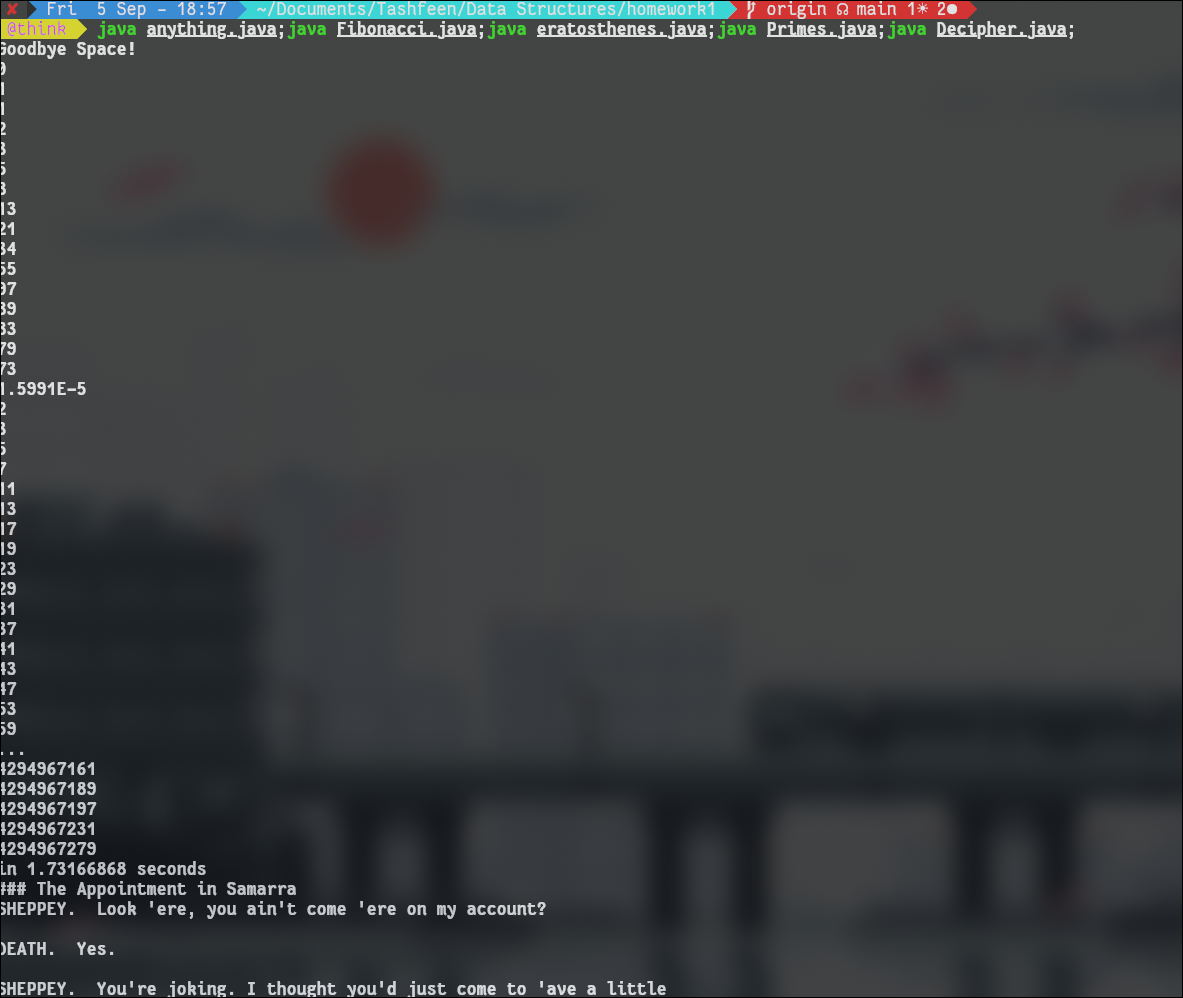
\includegraphics[width=\linewidth]{/home/think/Documents/Tashfeen/latex/Screenshot_05-Sep_18-58-23_31657.png}
% \end{figure}

% \begin{figure}
%   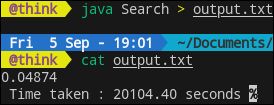
\includegraphics[width=\linewidth]{/home/think/Documents/Tashfeen/latex/Screenshot_05-Sep_19-02-32_7776.png}
% \end{figure}

\end{document}
